\begin{center}
\textbf{Содержание отчета}
\end{center}

\tableofcontents
\clearpage

\section{Введение и цель практики}

Производственная практика была посвящена анализу и систематизации результатов проекта по разработке рекомендательной системы выбора следующей культуры в севообороте. Практическая цель состояла не в создании полного агрономического оптимизатора, а в построении объяснимого рекомендательного прототипа, который по истории конкретного поля и базовому региональному контексту формирует краткий список вероятных следующих культур.

Актуальность рассматриваемой темы связана с тем, что задача выбора следующей культуры в севообороте на практике редко сводится к одному простому правилу. На решение одновременно влияют история конкретного поля, особенности региона, накопленные переходные закономерности между культурами и необходимость интерпретировать полученный результат. В этих условиях особенно полезен не жесткий автоматический выбор одной культуры, а инструмент, который помогает сузить пространство вариантов и показать наиболее правдоподобные кандидаты.

В ходе практики решались три взаимосвязанные задачи. Во-первых, необходимо было построить и проверить воспроизводимость исследовательского пайплайна: от предобработки данных до выбора финальной модели. Во-вторых, требовалось последовательно описать ключевые этапы работы и полученные результаты. В-третьих, важно было представить результаты в форме, пригодной для последовательного анализа и обсуждения.

Содержательно работа была сосредоточена на тех этапах проекта, которые формируют основное предиктивное ядро: подготовке данных, построении оконной выборки, сравнении простых и вероятностных baseline-подходов, обучении baseline-модели CatBoost и проверке промежуточной гипотезы о возможности улучшить результат с помощью графового сигнала переходов. Такое ограничение по содержанию позволяет сохранить целостность отчета и при этом показать логику выбора финальной модели.

\SourceNote

\section{Постановка задачи}

Рассматриваемая задача формулируется как рекомендация следующей культуры по краткой истории использования поля. Для каждого поля используются культуры за три предыдущих года и набор контекстных признаков:

\begin{center}
\(
(\mathrm{history}_1,\mathrm{history}_2,\mathrm{history}_3, x) \rightarrow \mathrm{target},
\)
\end{center}

где \texttt{history\_1}, \texttt{history\_2}, \texttt{history\_3} обозначают последовательность культур, а $x$ включает региональные и пространственные признаки поля. В отличие от обычной top-1 классификации, в проекте важен рекомендательный режим: модель должна не только предсказать наиболее вероятную культуру, но и сформировать содержательный список кандидатов.

Такая постановка принципиально отличается от полной задачи планирования севооборота. Полный оптимизационный подход требует учитывать большее число ограничений: экономику хозяйства, свойства почвы, погодные факторы, ресурсы техники, долгосрочные агротехнические ограничения и многие другие параметры. В данном проекте такая всеобъемлющая постановка сознательно не ставится. Вместо этого исследуется более узкая, но практически полезная задача: по уже имеющимся историческим данным поля сформировать правдоподобную рекомендацию следующего шага.

Именно поэтому отчет использует формулировку «прототип поддержки принятия решений». В этом режиме система не подменяет специалиста и не обещает гарантированно оптимальный выбор. Ее цель состоит в том, чтобы:
\begin{itemize}[leftmargin=1.5em]
\item структурировать историческую информацию о поле;
\item оценить вероятности возможных следующих культур;
\item показать, насколько модель выигрывает у простых ориентиров;
\item дать основу для дальнейшей интерпретации полученного результата.
\end{itemize}

На уровне архитектуры рассматриваемый фрагмент работы можно представить как переход от исходных данных через подготовку и обучение модели к итоговому предиктивному ядру. Эта логика отражена на рисунке~\ref{fig:practice-architecture}.

\begin{figure}[htbp]
\centering
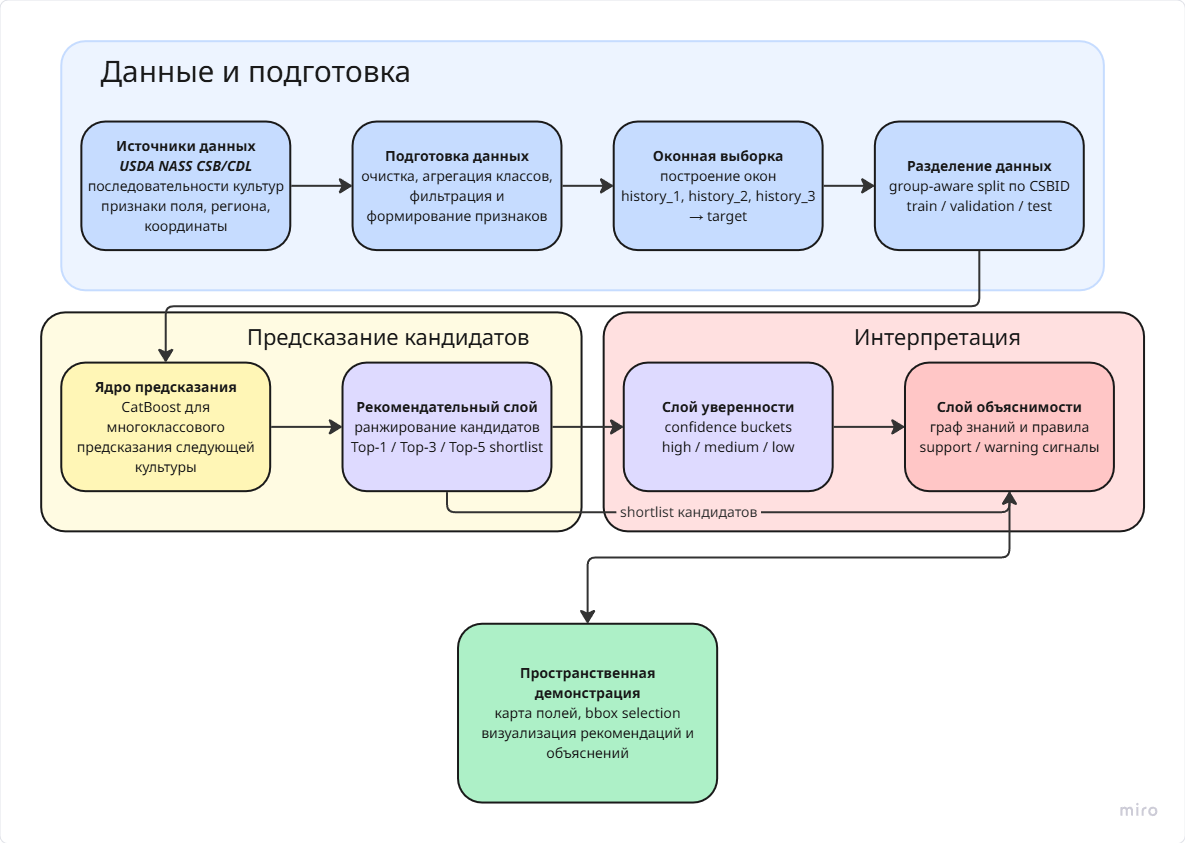
\includegraphics[width=0.88\textwidth]{../../diploma/crop-rotation/figures/architecture.png}
\caption{Общая схема исследовательского решения}
\label{fig:practice-architecture}
\end{figure}

В рамках практического отчета акцент сделан именно на этом ядре решения: подготовке данных, выборе baseline-модели и проверке исследовательской гипотезы о возможности усиления CatBoost графовым сигналом переходов между культурами.

\section{Данные и подготовка выборки}

\subsection{Источник данных}

В работе используются данные \textbf{USDA NASS CSB/CDL} за 2017--2024 годы. Слой CDL предоставляет годовые классы культур, а CSB служит источником идентификаторов полей, площади и пространственного контекста. Такой источник данных позволяет перейти от абстрактной региональной классификации к анализу последовательностей использования конкретных полей.

Практическая ценность такого набора данных состоит в том, что он соединяет два вида информации. С одной стороны, доступны последовательности культур по годам, а значит, можно анализировать смену культур во времени. С другой стороны, сохраняется привязка к конкретным полям и регионам, что позволяет не терять пространственный контекст наблюдений. Для задачи рекомендации следующей культуры это существенно: одинаковая история может интерпретироваться по-разному в зависимости от масштаба и положения поля.

\subsection{Предобработка и оконное представление}

На первом этапе исходные записи были приведены к интерпретируемому виду: CDL-коды культур сопоставлялись с названиями и укрупненными группами, после чего из выборки исключались нерелевантные для задачи категории. После базовой очистки подготовленный датасет содержит \PreparedRows{} строк.

Следующий этап заключался в преобразовании годовых последовательностей в оконное представление вида \texttt{history\_1, history\_2, history\_3 -> target}. Благодаря этому одна исходная история поля порождает несколько перекрывающихся обучающих окон, а задача приобретает форму предсказания следующего шага в последовательности культур. Полный window dataset содержит \WindowRows{} строк.

Смысл этого преобразования состоит в том, что модель начинает работать не с отдельным годом как изолированным наблюдением, а с короткой историей. Для каждого окна фиксируются три предыдущих значения культур и одна следующая культура, которую необходимо предсказать. В результате появляется естественная учебная постановка, близкая к задаче рекомендовать следующий элемент последовательности. Схема такого преобразования показана на рисунке~\ref{fig:practice-windows}.

\begin{figure}[htbp]
\centering
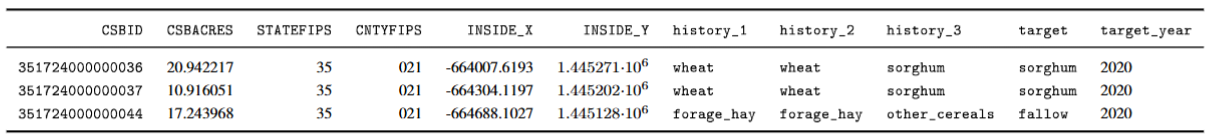
\includegraphics[width=0.92\textwidth]{../../diploma/crop-rotation/figures/windows.png}
\caption{Переход от годовых наблюдений к оконной постановке}
\label{fig:practice-windows}
\end{figure}

Этот шаг особенно важен для всей дальнейшей работы, потому что именно он связывает предметную постановку с формой, пригодной для машинного обучения. Если бы модель использовала только последний год, она сильнее напоминала бы простую модель переходов. Использование трехлетней истории позволяет учесть более длинные паттерны повторяемости и смены культур.

\subsection{Фильтрация классов и split}

Для стабилизации многоклассовой постановки редкие целевые классы были отфильтрованы, и итоговое пространство целей было сокращено до \TargetClasses{} культурных классов: \texttt{corn}, \texttt{cotton}, \texttt{fallow}, \texttt{forage\_hay}, \texttt{legumes}, \texttt{other\_cereals}, \texttt{sorghum}, \texttt{soybeans}, \texttt{wheat}. После фильтрации в выборке осталось \FilteredRows{} строк.

Фильтрация редких целевых классов была необходима не только для уменьшения дисбаланса, но и для сохранения устойчивой области применимости модели. Если оставить все исходные классы, то значительная часть из них будет представлена слишком малым числом наблюдений, что делает сравнительный анализ менее надежным и ухудшает интерпретируемость результатов. В результате проект сознательно сосредоточен на устойчивом наборе классов, который достаточно широко представлен в данных.

Разделение на обучающую, валидационную и тестовую выборки было выполнено как \textbf{group-aware split по \texttt{CSBID}}. Это означает, что окна, относящиеся к одному и тому же полю, не попадают одновременно в разные части выборки, что уменьшает риск утечки информации. Используется фиксированное значение \texttt{random\_state=42}. Итоговые размеры выборок составляют \TrainRows{} строк для train, \ValRows{} для validation и \TestRows{} для test.

Именно здесь формируется один из ключевых контрактов проекта. Если бы окна одного и того же поля оказались и в обучении, и в тесте, то итоговая оценка качества была бы завышенной: модель частично «узнавала» бы уже виденные истории. Групповое разбиение по \texttt{CSBID} устраняет этот риск и делает дальнейшее сравнение моделей методически корректным. Визуально структура такого разбиения приведена на рисунке~\ref{fig:practice-dataset-split}.

\begin{table}[htbp]
\centering
\small
\caption{Ключевые размеры выборок на этапах подготовки данных}
\label{tab:practice-data-sizes}
\begin{tabularx}{0.96\textwidth}{L{0.27\textwidth} r L{0.20\textwidth} X}
\toprule
Этап & Размер, строк & Источник & Комментарий \\
\midrule
Подготовленный датасет & 8 110 870 & \texttt{01\_meta.json} & Таблица после первичной очистки и приведения культурных кодов к рабочему виду \\
Оконный датасет & 40 554 350 & \texttt{02\_meta.json} & Набор формата \texttt{history\_1, history\_2, history\_3 -> target} \\
Итоговый датасет после фильтрации & 38 511 210 & \texttt{02\_meta.json} & Оконная выборка после исключения редких целевых классов \\
Train & 26 957 630 & служебные метаданные проекта & Обучающая часть фиксированного разбиения по \texttt{CSBID} \\
Validation & 5 776 566 & служебные метаданные проекта & Валидационная часть того же разбиения \\
Test & 5 777 014 & служебные метаданные проекта & Тестовая часть того же разбиения \\
\bottomrule
\end{tabularx}
\end{table}


\begin{figure}[htbp]
\centering
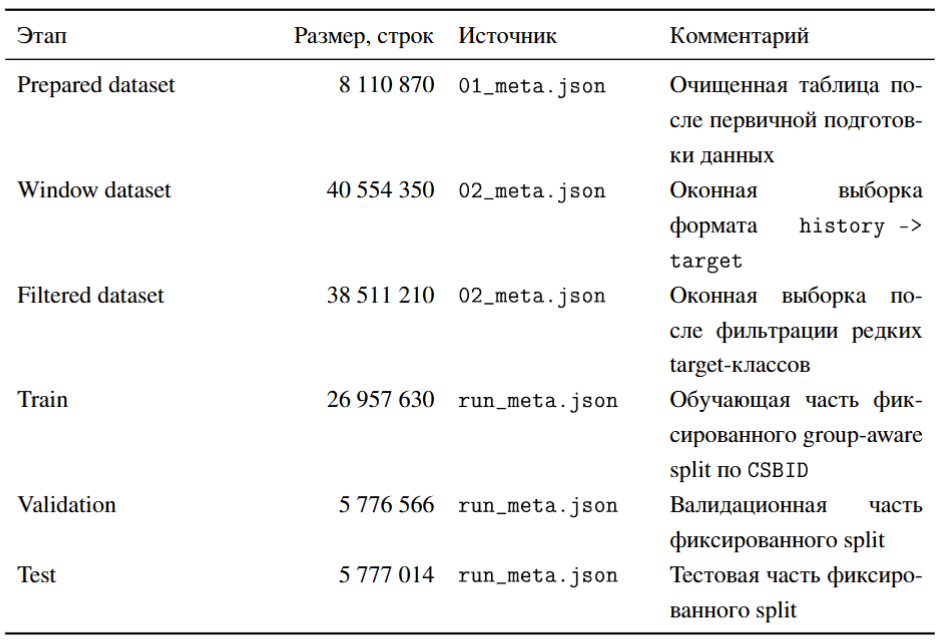
\includegraphics[width=0.92\textwidth]{../../diploma/crop-rotation/figures/dataset_split.png}
\caption{Схема фиксированного разбиения выборки}
\label{fig:practice-dataset-split}
\end{figure}

\section{Формирование признаков и frozen split}

Финальная baseline-модель использует компактный и интерпретируемый набор признаков:
\begin{itemize}[leftmargin=1.5em]
\item история культур за три предыдущих года: \texttt{history\_1}, \texttt{history\_2}, \texttt{history\_3};
\item региональные признаки: \texttt{STATEFIPS}, \texttt{CNTYFIPS};
\item характеристики поля: \texttt{CSBACRES};
\item пространственный контекст: \texttt{INSIDE\_X}, \texttt{INSIDE\_Y}.
\end{itemize}

Такой набор признаков отражает основную гипотезу проекта: следующая культура зависит не только от последней культуры, но и от более длинной локальной истории, а также от региона и базовых пространственных характеристик участка. При этом признаки остаются достаточно простыми, чтобы пайплайн был воспроизводимым и удобным для дальнейшего сравнения с baseline-подходами.

Каждый из этих признаков играет отдельную роль. Исторические признаки дают модели информацию о последовательности смены культур. Региональные коды помогают учитывать различия между территориями, которые могут быть связаны с региональной специализацией и сложившимися паттернами возделывания. Площадь поля позволяет модели использовать очень грубую, но полезную характеристику масштаба участка. Пространственные координаты дополняют региональный контекст более непрерывным описанием положения поля.

\begin{table}[htbp]
\centering
\small
\caption{Признаки финальной baseline-модели CatBoost}
\label{tab:practice-final-features}
\begin{tabularx}{0.96\textwidth}{L{0.22\textwidth} L{0.18\textwidth} X}
\toprule
Признак & Тип & Смысл \\
\midrule
\texttt{history\_1} & категориальный & Культура в первом году исторического окна поля \\
\texttt{history\_2} & категориальный & Культура во втором году исторического окна поля \\
\texttt{history\_3} & категориальный & Культура в ближайшем к целевому году исторического окна \\
\texttt{STATEFIPS} & категориальный & Код штата как общий региональный контекст \\
\texttt{CNTYFIPS} & категориальный & Код округа как более локальный региональный контекст \\
\texttt{CSBACRES} & числовой & Площадь поля по данным CSB \\
\texttt{INSIDE\_X} & числовой & Пространственная координата поля по оси X \\
\texttt{INSIDE\_Y} & числовой & Пространственная координата поля по оси Y \\
\bottomrule
\end{tabularx}
\end{table}


Зафиксированное разбиение по \texttt{CSBID} является важной частью исследовательского контракта. Благодаря frozen split все модели и эксперименты оцениваются на одном и том же разделении данных, а сравнение baseline-подходов, CatBoost и graph-гибрида остается корректным. Фиксация \texttt{random\_state=42} здесь также важна: она гарантирует, что при повторном обращении к этим этапам сохраняется одна и та же логика разбиения, а результаты разных моделей сопоставимы не только содержательно, но и технически.

Таким образом, на данном этапе формируется компактное, но устойчивое представление задачи. Оно достаточно информативно для обучения модели и достаточно прозрачно для анализа, что особенно важно в исследовательском контексте практического отчета.

\section{Базовые методы и выбор финальной модели}

\subsection{Baseline-подходы}

До перехода к CatBoost были рассмотрены несколько ориентировочных baseline-моделей. Стратегия \texttt{most\_frequent} всегда выбирает самый частый класс обучающей выборки и задает нижнюю границу качества. Стратегия \texttt{last\_crop} повторяет последнюю наблюдаемую культуру в истории поля и позволяет оценить, насколько полезен простой инерционный сценарий.

Дополнительно использовался вероятностный baseline \texttt{Markov-1}, основанный на одношаговой модели переходов:
\begin{center}
\(
P(\mathrm{target}\mid\mathrm{history}_3).
\)
\end{center}

Этот подход уже учитывает статистику переходов между культурами, но по-прежнему игнорирует более длинную историю и дополнительные признаки региона и поля. На test \texttt{Markov-1} показывает Accuracy \MarkovAcc{}, Macro F1 \MarkovMacroFOne{} и Weighted F1 \MarkovWeightedFOne{}.

Сравнение этих ориентиров важно не само по себе, а как способ понять, какой вклад дают разные уровни сложности модели. Если бы результат CatBoost был близок к \texttt{most\_frequent}, это означало бы, что задача фактически сводится к доминированию нескольких частых классов. Если бы CatBoost был близок к \texttt{last\_crop}, это бы говорило о сильной инерционности последовательностей. Если бы он почти не выигрывал у \texttt{Markov-1}, то можно было бы заключить, что одной последней культуры в истории почти достаточно для предсказания.

\subsection{Финальная baseline-модель CatBoost}

Финальным предиктивным ядром проекта является baseline-версия CatBoost. Выбор этой модели обусловлен табличной природой задачи и сочетанием категориальных и числовых признаков. CatBoost использует компактный набор признаков и возвращает вероятности по всем целевым классам, что делает модель пригодной как для top-1 предсказания, так и для рекомендательного режима.

На test baseline CatBoost показывает следующие значения:
\begin{itemize}[leftmargin=1.5em]
\item Accuracy = \BaselineAcc{};
\item Macro F1 = \BaselineMacroFOne{};
\item Weighted F1 = \BaselineWeightedFOne{}.
\end{itemize}

Полученные значения существенно превосходят простые baseline-подходы и подтверждают, что использование трехлетней истории вместе с региональным и пространственным контекстом дает устойчивый выигрыш в качестве. Именно поэтому модель \FinalModel{} зафиксирована как финальная и рассматривается как основа рассматриваемого решения.

Практически это означает, что baseline CatBoost извлекает из данных больше информации, чем простые правила и даже одношаговая вероятностная модель переходов. Модель использует не только ближайшую культуру, но и более длинный исторический контекст, а также сведения о положении и масштабе поля. За счет этого она лучше различает ситуации, где несколько культур выглядят правдоподобно, но их вероятности должны быть расставлены по-разному.

На рисунке~\ref{fig:practice-baseline-comparison} и в таблице~\ref{tab:practice-model-comparison} показано, что baseline CatBoost устойчиво опережает остальные базовые варианты. Это и стало главным аргументом в пользу выбора именно этой модели как финального предиктивного ядра.

\begin{figure}[htbp]
\centering
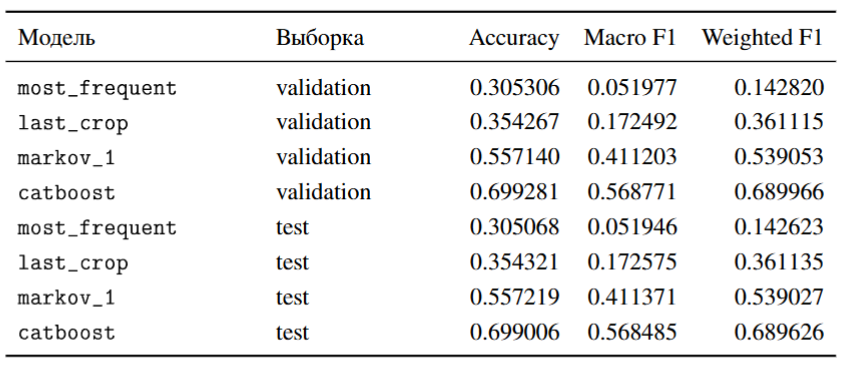
\includegraphics[width=0.88\textwidth]{../../diploma/crop-rotation/figures/comparison_baseline.png}
\caption{Сравнение baseline-подходов и baseline-модели CatBoost}
\label{fig:practice-baseline-comparison}
\end{figure}

\begin{table}[htbp]
\centering
\scriptsize
\caption{Сравнение baseline-подходов и основных CatBoost-экспериментов на test-выборке}
\label{tab:practice-model-comparison}
\begin{tabularx}{0.98\textwidth}{L{0.24\textwidth} X r r r}
\toprule
Подход & Краткая характеристика & Accuracy & Macro F1 & Weighted F1 \\
\midrule
\texttt{most\_frequent} & Всегда выбирается самый частый класс обучающей выборки & 0.305068 & 0.051946 & 0.142623 \\
\texttt{last\_crop} & Следующая культура приравнивается к последней наблюдаемой культуре поля & 0.354321 & 0.172575 & 0.361135 \\
\texttt{Markov-1} & Одношаговая вероятностная модель переходов вида $P(\mathrm{target}\mid\mathrm{history}_3)$ & 0.557219 & 0.411371 & 0.539027 \\
Baseline CatBoost & История, регион, площадь и координаты поля & 0.699006 & 0.568485 & 0.689626 \\
CatBoost + extra features & Дополнительные признаки истории: разнообразие культур, индикаторы повторяемости, наличие отдельных групп культур & 0.699235 & 0.569473 & 0.689991 \\
CatBoost + transition graph & Гибридная оценка $\alpha p_{\mathrm{catboost}}+\beta p_{\mathrm{graph}}$ с лучшей конфигурацией $\alpha=0.9$, $\beta=0.1$ & 0.698714 & 0.564387 & 0.688729 \\
\bottomrule
\end{tabularx}
\end{table}


\section{Эксперимент CatBoost + transition graph}

После обучения baseline-модели была проверена гипотеза о том, что ранжирование кандидатов можно улучшить за счет графового сигнала переходов между культурами. Для этого рассматривалась гибридная оценка:
\begin{center}
\(
\mathrm{score}=\alpha \cdot p_{\mathrm{catboost}}+\beta \cdot p_{\mathrm{graph}},
\)
\end{center}

где $p_{\mathrm{catboost}}$ --- вероятность, рассчитанная моделью CatBoost, а $p_{\mathrm{graph}}$ --- сигнал графа переходов. Проверялись несколько сочетаний весов; лучшим вариантом оказался $\alpha=\GraphAlpha$ и $\beta=\GraphBeta$.

Смысл этого эксперимента заключался в проверке следующей гипотезы: если в данных присутствуют устойчивые переходы между культурами, то отдельный графовый сигнал может помочь улучшить модельное ранжирование. В таком случае вероятности CatBoost и оценки переходов не конкурировали бы друг с другом, а взаимно дополнялись. На уровне идеи это выглядело вполне правдоподобно, поскольку проект изначально связан с анализом последовательностей культур.

Однако даже в лучшей конфигурации гибридный вариант уступил чистому CatBoost. На test были получены Accuracy \GraphAcc{}, Macro F1 \GraphMacroFOne{} и Weighted F1 \GraphWeightedFOne{}. Разница невелика, но она показывает, что простое переранжирование на основе графового сигнала не дает достаточных оснований для смены финальной модели.

Этот отрицательный результат имеет важное исследовательское значение. Во-первых, он показывает, что baseline CatBoost уже достаточно хорошо извлекает переходные закономерности из исходного представления данных, и простой внешний графовый сигнал не дает автоматического выигрыша. Во-вторых, он помогает развести в проекте две разные роли: предсказание и интерпретацию. Если графовый компонент не улучшает качество как самостоятельная добавка к ранжированию, его разумнее использовать не как замену модели, а как дополнительный аналитический слой для объяснения результата.

Таким образом, эксперимент \texttt{CatBoost + transition graph} остается важной частью исследовательской логики проекта, но не меняет финальный выбор. Он показывает, что проверка даже неудачной гипотезы полезна, если она помогает лучше понять границы применимости выбранной модели и уточнить архитектуру решения.

\section{Заключение}

В ходе производственной практики были систематизированы ключевые результаты проекта, посвященного рекомендации следующей культуры по истории поля. Подтверждена воспроизводимая структура исследовательского пайплайна: от очистки исходных данных и построения оконной выборки до выбора финальной модели и проверки промежуточных экспериментальных веток.

Главным результатом работы стало последовательное описание проекта как объяснимого рекомендательного прототипа поддержки принятия решений. В текст отчета включены только основные этапы до эксперимента \texttt{CatBoost + transition graph}, что позволяет сохранить разумный объем и при этом показать логику выбора финальной модели \FinalModel{}.

В ходе работы было показано, что путь от исходных данных до финальной модели включает несколько принципиально важных решений: выбор рабочей формы данных, фильтрацию пространства классов, корректное разбиение по полям, сравнение с простыми ориентирами и проверку промежуточных экспериментальных гипотез. Благодаря этому выбор baseline CatBoost выступает не как декларация, а как результат последовательного сравнения моделей и анализа их поведения.

Дальнейшее развитие проекта включает более поздние этапы, связанные с рекомендательной оценкой, анализом уверенности, объяснимым графовым слоем и пространственной демонстрацией. В настоящем отчете эти направления не раскрываются подробно, поскольку основной задачей было зафиксировать базовое исследовательское ядро рассматриваемого решения.
